\documentclass[11pt,british]{article}
\usepackage[T1]{fontenc}
\usepackage[latin9]{inputenc}
\usepackage{lmodern}
\usepackage{geometry}
\usepackage{graphicx}
\usepackage{pdfpages}
\usepackage{lscape}
\usepackage{listings}
\lstset{language=VHDL}
\usepackage{babel}
\usepackage[justification=centering]{caption}
\usepackage{float}

%%%%%%%%%%%%%%%%%%%%%%%%%%%%%%
\usepackage{afterpage}
\newcommand\blankpage{%
    \null
    \thispagestyle{empty}%
    \addtocounter{page}{-1}%
    \newpage}
%%%%%%%%%%%%%%%%%%%%%%%%%%%%%%

\geometry{verbose,tmargin=2.5cm,bmargin=2.5cm,lmargin=2.5cm,rmargin=2.5cm,headheight=2.1cm}
\exhyphenpenalty=10000\hyphenpenalty=10000
\makeatletter
\makeatother

%%%%%%%%%%%%%%%%%%%%%%%%%%%%%%%%%%%%%%%%%%%%%%%%%%%%%%%%%%%%
%% Title- & blank page
\begin{document}

%%Mandatory blank page
\newpage
\thispagestyle{empty}
\mbox{}

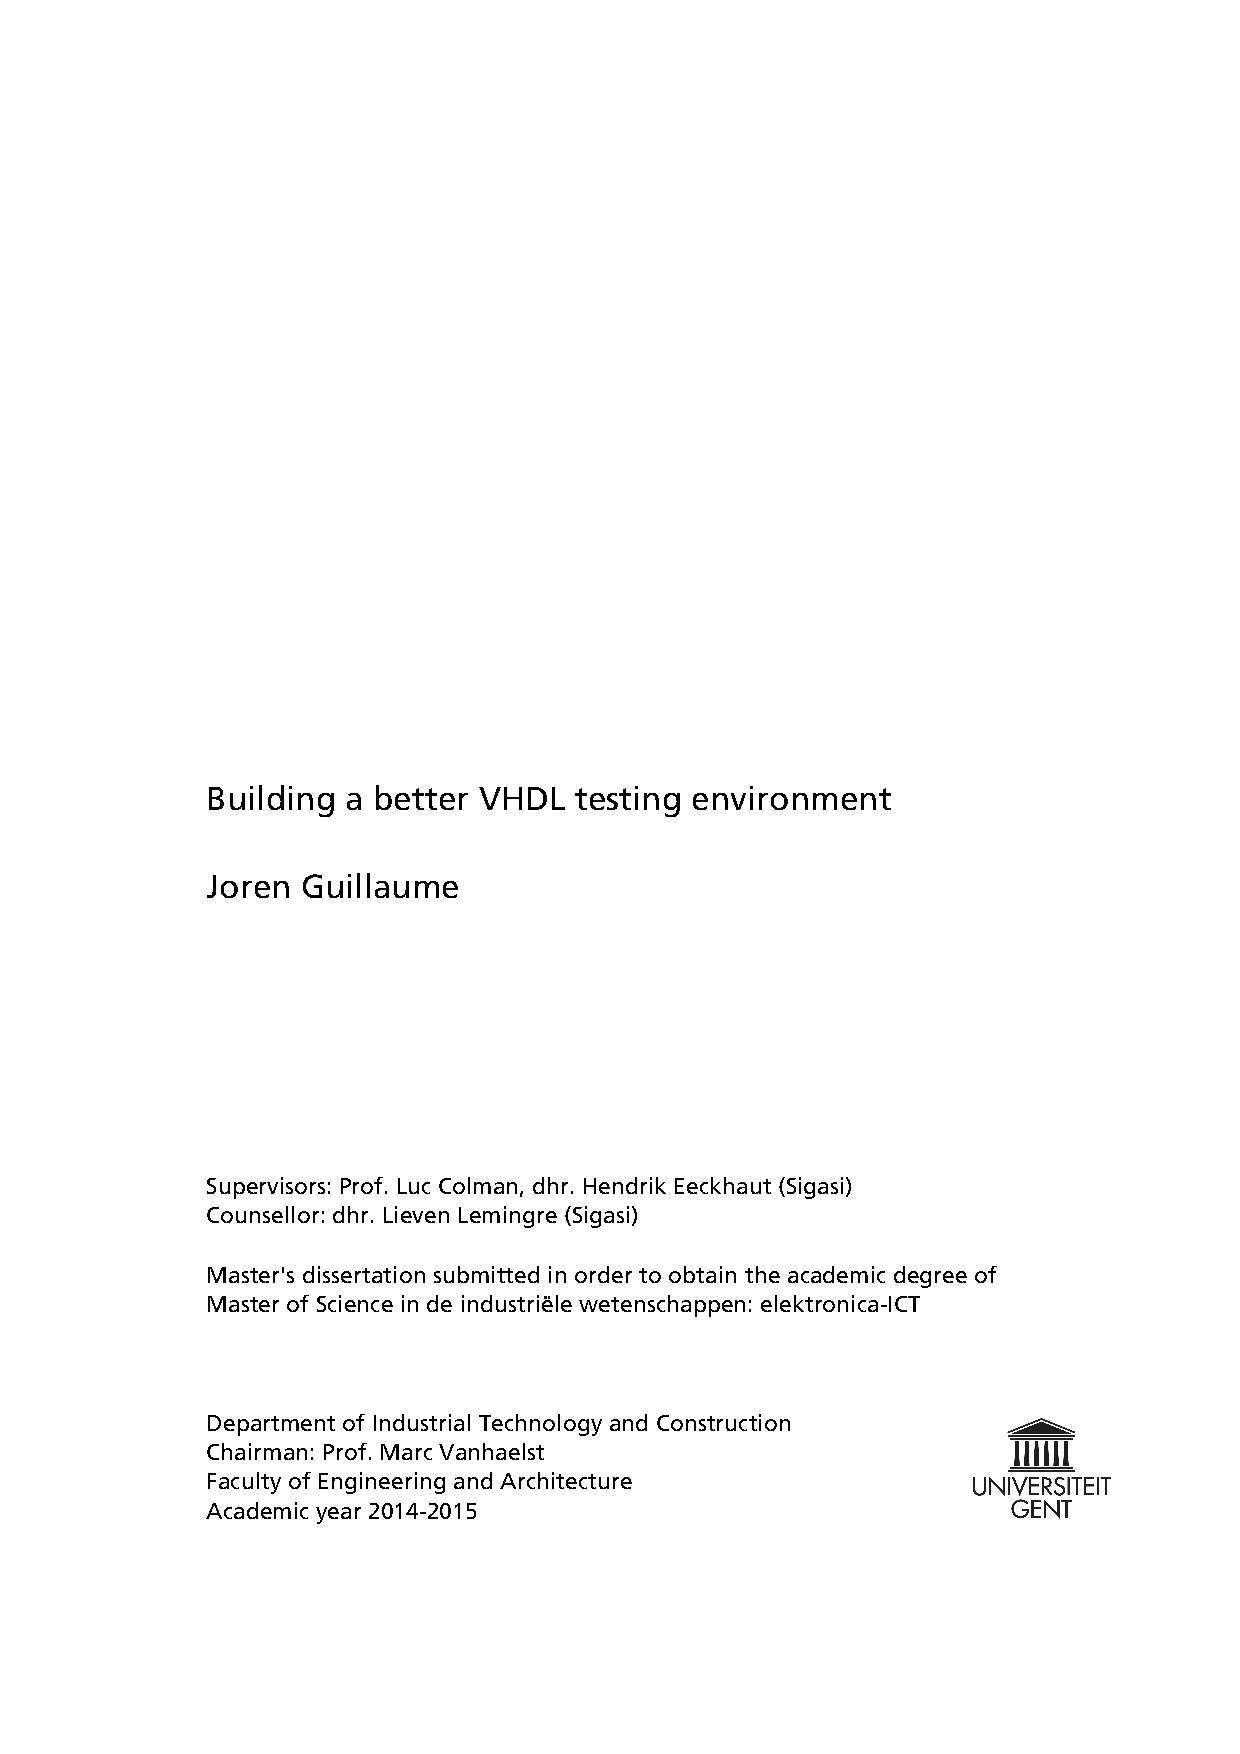
\includepdf[pages={1}]{title-generated.pdf}

%%%%%%%%%%%%%%%%%%%%%%%%%%%%%%%%%%%%%%%%%%%%%%%%%%%%%%%%%%%%
%% Copyright notice

\newpage{}\part*{Usage restrictions}

The author gives permission to make this master dissertation available for consultation 
and to copy parts of this master dissertation for personal use. 
 In the case of any other use, the copyright terms have to be respected, in particular with regard to 
the obligation to state expressly the source when quoting results from this master dissertation.

\pagebreak{}

%%%%%%%%%%%%%%%%%%%%%%%%%%%%%%%%%%%%%%%%%%%%%%%%%%%%%%%%%%%%
%% Preface

\newpage{}\part*{Preface}

\pagebreak{}

%%%%%%%%%%%%%%%%%%%%%%%%%%%%%%%%%%%%%%%%%%%%%%%%%%%%%%%%%%%%
%% Abstract

\newpage{}
\begin{abstract}
\end{abstract}

%%%%%%%%%%%%%%%%%%%%%%%%%%%%%%%%%%%%%%%%%%%%%%%%%%%%%%%%%%%%
%% Extended abstract

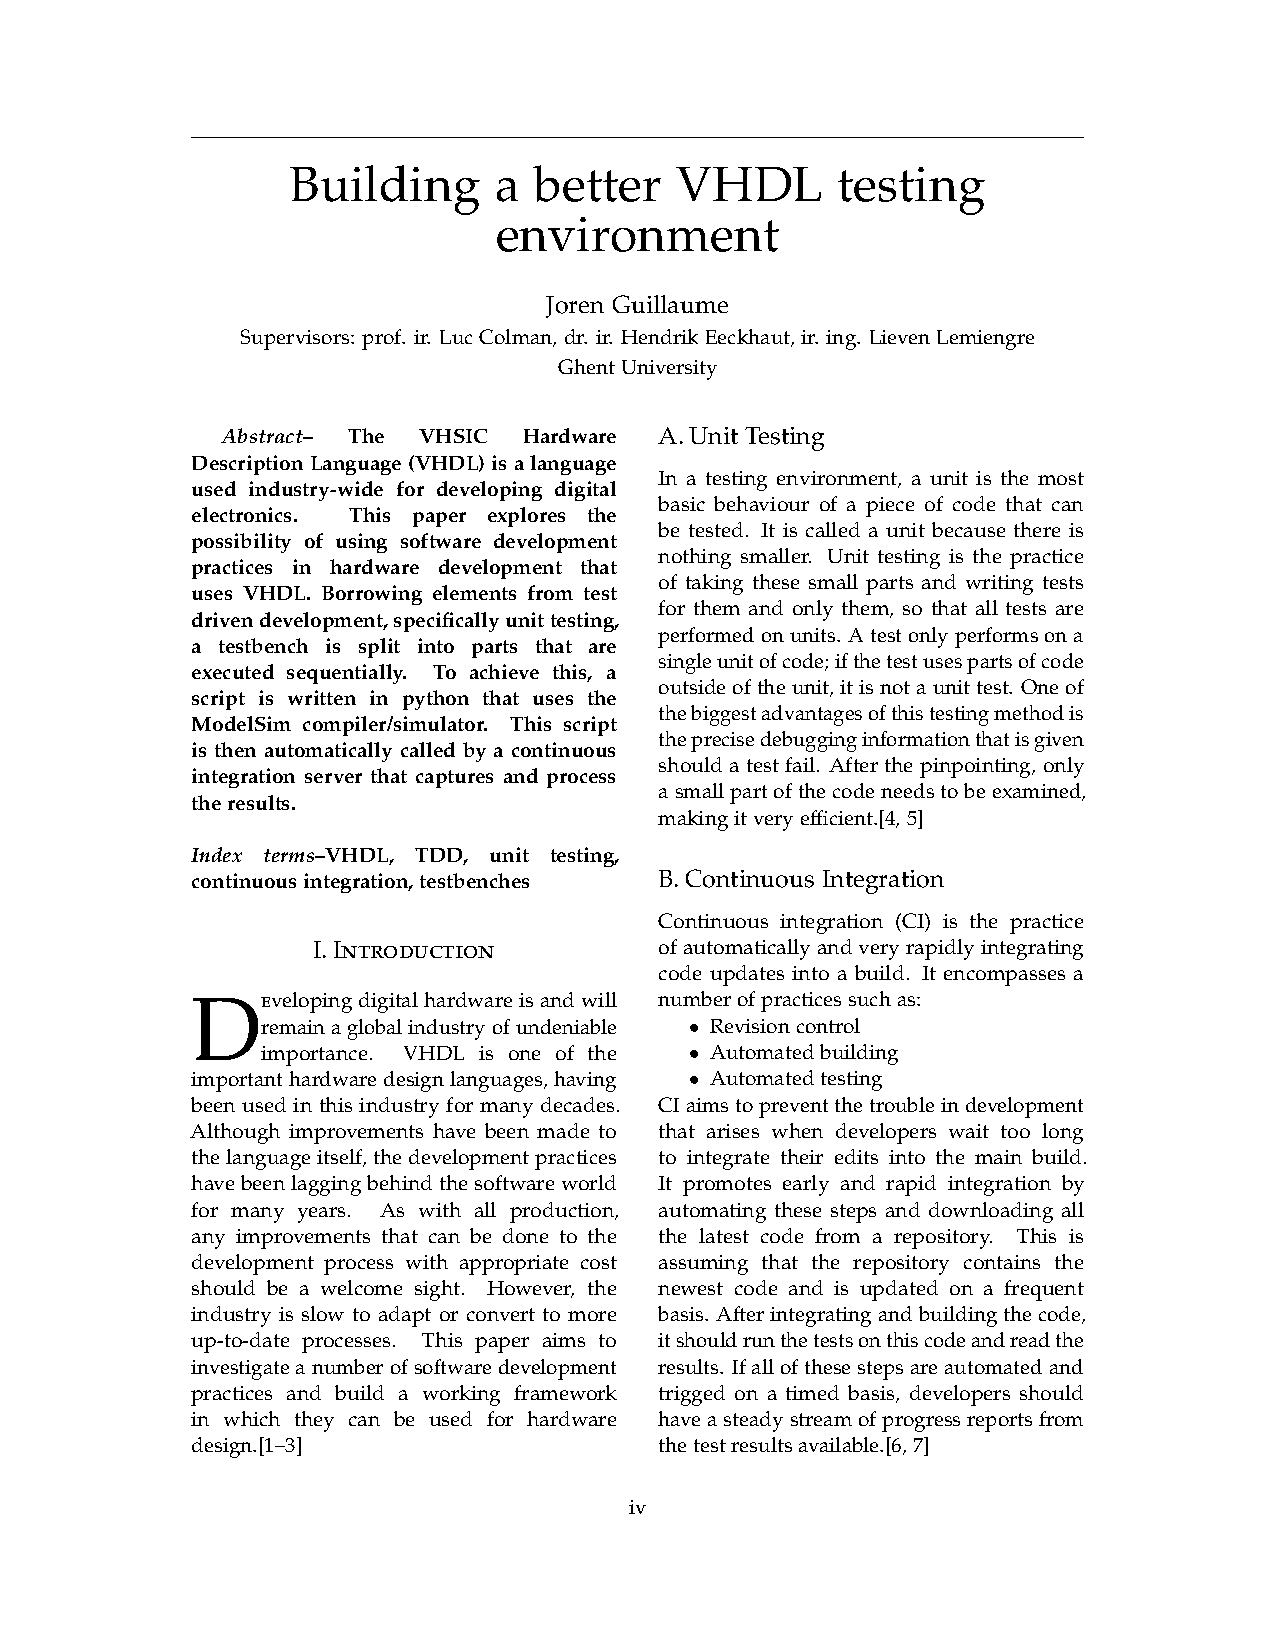
\includepdf[pages={1,2}]{extended-abstract.pdf}

%%%%%%%%%%%%%%%%%%%%%%%%%%%%%%%%%%%%%%%%%%%%%%%%%%%%%%%%%%%%
%% Table of Contents

\tableofcontents
\pagebreak

%%%%%%%%%%%%%%%%%%%%%%%%%%%%%%%%%%%%%%%%%%%%%%%%%%%%%%%%%%%%
%% List of figures

\listoffigures
\pagebreak

%%%%%%%%%%%%%%%%%%%%%%%%%%%%%%%%%%%%%%%%%%%%%%%%%%%%%%%%%%%%
%% List of tables

\listoftables
\pagebreak

%%%%%%%%%%%%%%%%%%%%%%%%%%%%%%%%%%%%%%%%%%%%%%%%%%%%%%%%%%%%
%% Used abbreviations and acronyms

\section*{List of Acronyms and Abbreviations}
\pagebreak

%%%%%%%%%%%%%%%%%%%%%%%%%%%%%%%%%%%%%%%%%%%%%%%%%%%%%%%%%%%%

\part{Problem and background}


\section{Problem}

Developing VHDL, like any code, is prone to error creation, either by user or by wrong product specifications. To ensure errors are weeded out before the more expensive production begins, the code must be subjected to rigorous testing. Currently, large and impractical tests are needed to fully test a product.
\\
\\
Because testing is such a time consuming process, finding errors often
results in severe delays due to the need to both correct the error
and test for others. Therefore it is in the best interests of both
testing- and software engineers to find and correct errors
with minimal delay and maximal efficiency. This process should affect
the least amount of code possible in order to minimize time spent retesting
and modifying the code.
\\
\\
In this thesis, a number of mechanics are used to optimize both testing and coding. Based loosely off of Test Driven Development (TDD), tests are written to function and be tested independently.  In order to maximize coverage and keep the time spent writing tests to a minimum, a library with often used functions and other useful code is made available. Alongside of it is a tool, written in Python, to process tests independently  and represent the results in a quick and easy-to-read format.


\newpage{}


\section{Introduction}
\label{sec:intro}

\subsection{Digital Electronics}

There are two kinds of electronic appliances and circuits; digital and analogue. Digital electronics differ from analogue electronics in that they use a discrete set of voltage levels to transmit signals. The most common number of items in the set is 2, a level for one (commonly
named \emph{high}) and a level for zero (commonly named \emph{ground} or \emph{low}). The advantage of using a discrete number of levels rather than a continuous signal as is used in analogue electronics, is that noise generated by the environment, thermal noise and other interfering factors will have but a minor influence on the signal.
\\
\\
To process these discrete signals, electronics are made up of transistors that nowadays are formed in with the \emph{Complementary Metal Oxide Semiconductor }(CMOS) technology. This technology uses both an \emph{NPN} and a \emph{PNP} transistor that work in a push-pull configuration. The p's and n's in NPN and PNP simply stand for \emph{Positive} and \emph{Negative}. They are made of positively and negatively doped lumps of semiconductor (usually silicon-dioxide or SiO$_{2}$). A transistor is basically a blockage on a track and depending on the force applied to its \emph{gate}, it opens or closes the track.
\\
\\
In reality, the force takes the form of a current and an NPN transistor opens its gate when a positive current is applied. A PNP transistor, however, always leaves its gate open until a current is applied. This means that if we send the same signal to an NPN and a PNP transistor, with one of the signals inverted, we can open and close two parts of the entire circuit at the same time. This is useful to both direct a certain signal to ground and at the same time close its connection with the \emph{source} (the power source). Hence also the name \emph{Complementary} MOS, the NPN and PNP complement each other.
\\
\\
A certain combination of transistors is used to make \emph{logic gates}. These logic gates make sure that only a certain combination of ones and zeroes at the inputs result in certain ones or zeroes at the outputs. For instance, one of the most common logic gates is a \emph{nand }gate (a \emph{not and }gate). This gate has a number of inputs ranging from 2 to theoretically infinity (but practically 3 or 4) and only outputs a \emph{low} signal if all of the inputs are \emph{high} (digital one), otherwise its output is \emph{at ground} or \emph{low} (digital zero). The other most common logic gate is the \emph{nor }gate (a \emph{not or }gate). This gate outputs a low signal if any of its inputs are high, otherwise it outputs a low.
\\
\\
A common mistake is to think that low or ground mean \emph{zero voltage.} This is only partially true, the high signals are measured with ground as their reference. So a high signal of 1.8 V would be 1.8 V higher than ground, and could be considered to be at 1.8 V if ground is the theoretical zero. These logic gates are themselves combined to build higher-level blocks such as flip-flops, which are used to make registers and so on up to the entire chip design.

\pagebreak

\subsection{Hardware Description Languages}

A \emph{Hardware Description Language} (HDL) can be used to describe any one of the levels mentioned in the previous section, right down to the logic gate level. However, this last one is wholly unnecessary considering synthesis tools can produce superior logic gate-level layouts \cite{key-1}. The level that uses certain blocks of logic gates to describe more complex behaviour is called the \emph{Register Transfer Level} or RTL. Some blocks are standard implementations that have been widely used and are nearly fully optimized, such as memories, flip-flops and clocks. An RTL flip-flop implementation is shown here: 
\begin{lstlisting}[tabsize=4, frame=single, framesep=2mm, belowskip=16pt, aboveskip=16pt]
library IEEE;
use IEEE.std_logic_1164.all;
entity DFF is
	Port(D 	 : in std_logic;
		 CLK : in std_logic;
		 Q 	 : out std_logic;
end DFF;
architecture Behavioural of DFF is
begin
	process (CLK)
	begin
		if rising_edge(CLK) then
			Q <= D;
		end if;
	end process;
end Behavioural;
\end{lstlisting}

The IEEE library provides a number of extensions on the original VHDL specification that allow a more realistic simulation and description of hardware behaviour. An \emph{entity} defines the inputs and outputs of a certain building block, in this case the D Flip-flop or DFF. The D stands for Delay, and it simply puts on its output, Q, that which was on the input, D, one clock period earlier. The \emph{architecture}, in this case Behavioural, takes the description of an entity and assigns a real implementation to it. All \emph{processes} are executed in parallel, this does not mean that all are triggered at the same time, nor do they take equally as long to finish, but it means that any process can be executed alongside any other process. In this case there is only one (nameless) process that describes the entire behaviour of the flip-flop. The process waits for the rising edge of the clock, which is a transition from zero to one, after which it schedules the value of D to be put on Q when the next rising edge appears.
\\
\\
This is a basic example of an entity, an architecture and a process. This flip-flop could be used in certain numbers to build a \emph{register}, a collection of ones and zeroes (henceforth referred to as \emph{bits}) that is used to (temporarily) store these values. The register could then be used alongside combinational logic to build an even bigger entity. The idea here is that small building blocks can be combined to produce vast and complex circuits that are nearly impossible to describe in one go. Adding all these layers together also creates a lot of room for error, and having a multi-level design makes it challenging to pinpoint the exact level and location of any errors. Therefore, it is paramount that all code on all levels is tested thoroughly, which is done by use of \emph{testbenches} \cite{key-2}.
\\
\\
Testbenches are made up of code that takes a certain building block, the \emph{Unit Under Test} (UUT) or \emph{Device Under Test} (DUT). The testbench then puts a certain sequence of values on the inputs and monitors the outputs. If the device performs normally, the received output sequence should match a certain \emph{golden reference}, the expected output sequence. In these testbenches it is good practice to observe how well a device performs if its inputs behave outside of the normal mode of operation. When all of these tests have finished and the output performs as expected, the device is ready to be put into production or further down the developmental process.
\\
\\
If a device is not tested properly and faults propagate throughout development, they can be very expensive to correct, especially at the stage of production, where a single photomask, used to ``print'' part of the layout, can easily cost \$100,000 \cite{key-3}. Therefore a large portion of time is spent writing and executing tests\cite{key-4}. A large number of practices to improve both the speed and quality of testing and coding exist, but the focus chosen in this thesis is \emph{Test Driven Development} (TDD). This practice has proven to increase test coverage \cite{key-5}, decrease defect density \cite{key-8} as well as improve code quality \cite{key-8,key-9}.

\begin{figure}[h]
    \centering
	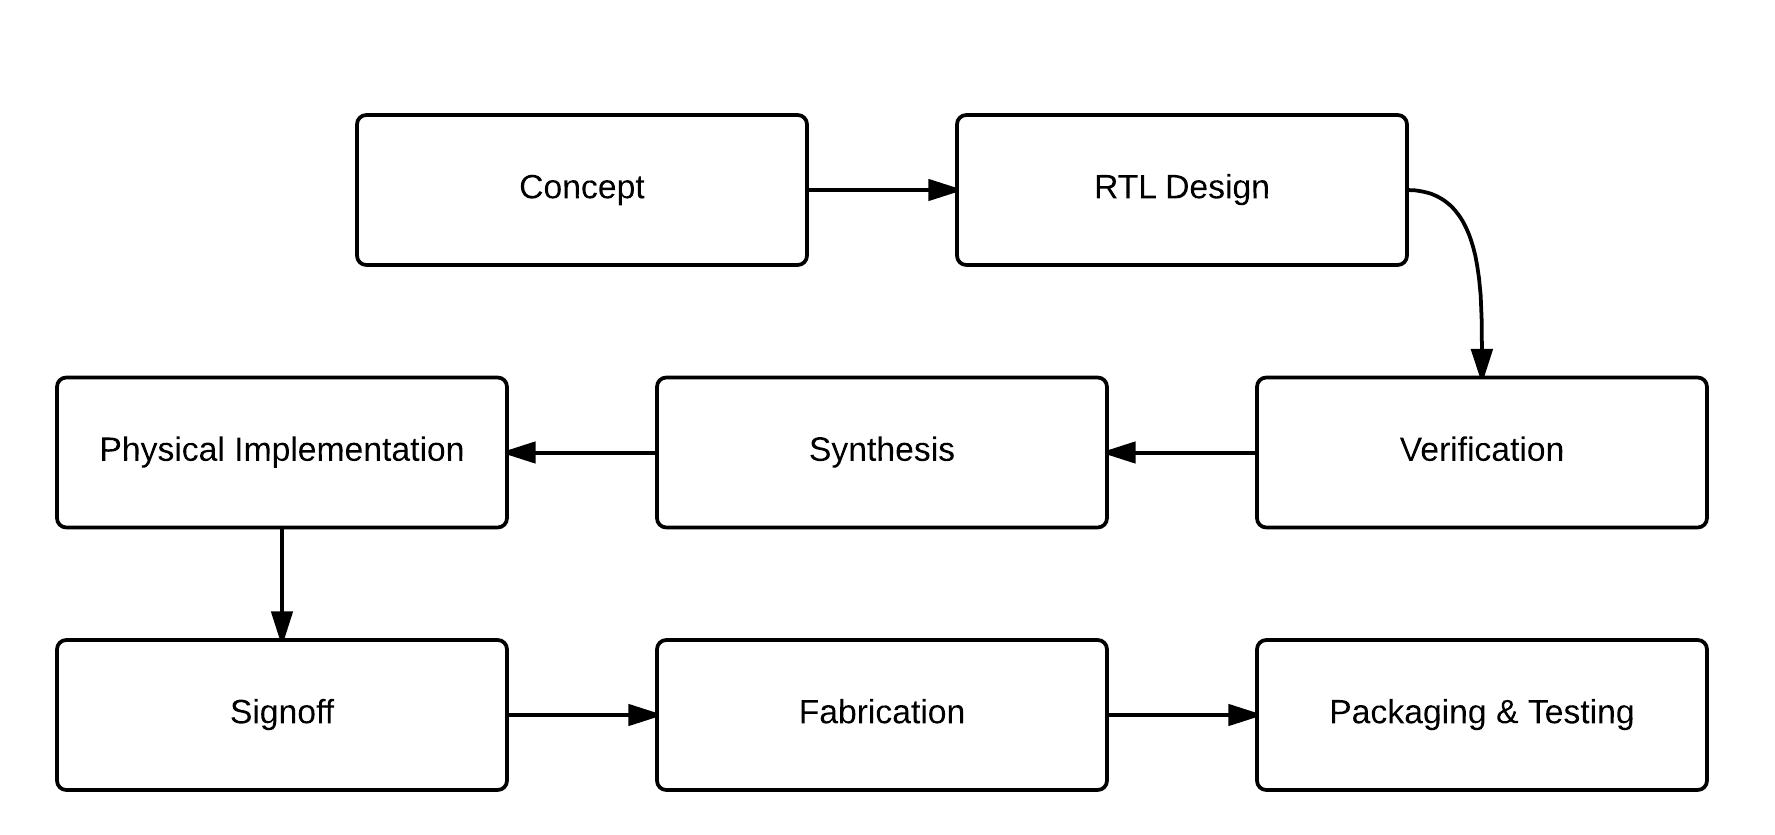
\includegraphics[width=\textwidth]{images/Design_Flow.png}
    \caption{Typical CMOS design flow}
    \label{fig:Design_Flow}
\end{figure}


\subsection{Test Driven Development}
Test Driven Development is a proven development technique that has regained traction in the past decade, primarily through the efforts of Kent Beck \cite{key-10}. The technique focuses on tests being created before the actual code. It is important to make certain distinctions before going more in depth on the used methods. The developing community has a great many practices, each with their own names and methods, and hardly none are mutually exclusive.

\subsubsection{Unit Testing}
To understand TDD, an basic knowledge of \emph{Unit Testing} is required. In software testing, a unit test is a test designed to check a single unit of code. Ideally, this unit is the smallest piece in which the code can be divided. A unit test should always test only a single entity, and only one aspect of that entity's behaviour. This division in units has a number of benefits, one of the most important being that code is exceedingly easy to maintain. Furthermore, the division of the code makes changes, when needed, fast to be carried out and ensures that only the modified code needs to re-tested.

\subsubsection{Test First Development}
Another main component of TDD is \emph{Test First Development}, a technique that has a developer writing tests first, before any code has been written. This method makes the developer think on what the code has to achieve, rather than what the specific implementation has to be. A key feature of a new test is that it has to fail during its first run. If not, the test is obsolete seeing as the functionality it tests has already been implemented. After being run for the first time (and failing), the developer implements just enough code to get the test to pass. Once the test succeeds, it is time for a new test.

\subsubsection{Refactoring}
The third pillar of TDD is refactoring. After the tests succeed, it is necessary to clean up the code. A well-done TFD implementation uses the bare amount of code needed to make the test pass, but this is of course usually not the best code possible. Refactoring means that you take existing code and modify only the code itself to perform better. This leaves both the input and output of the tests and code unchanged, only the way the code processes input is altered. It is important in this step to edit nothing in the test code or the outputs or inputs. Otherwise, either the test would behave differently or new tests would have to be written. The latter goes directly against the TFD principle.

\subsubsection{Test Driven Development}
Test Driven Development is a combination of the previously mentioned techniques. A Unit Test is written before any code, the test is then executed and should fail. After the failure, the most basic code to make the test pass is implemented, the test is then executed again and should pass. After this first pass, the code written for the passing of the test, and only this code, is edited to perform and look better. This follows all steps mentioned above, a \emph{Unit Test} is written according to \emph{Test First Development} and is \emph{Refactored} later.

\newpage

\section{Testing VHDL}
%Wat zijn de gangbare praktijken in de industrie?
%Wat is het marktaandeel van VHDL?
%Wat doet VHDL bij een testbench? Specialiteitjes waar er op gelet moet worden?
%Wat is de gemiddelde looptijd van een groot project?

\newpage

\section{Exploring solutions}
During the making of this thesis, a number of approaches was investigated and some were put to practical use. Ultimately, the most practical and straightforward approach was to implement a form of Unit Testing. Alongside, an extensive library, written in VHDL, was used to ease the building of testbenches. Finally, a central server was installed that repeatedly and automatically ran the script and read the resulting test outputs.

%Wat is CI? Wat doet Hudson?
%Kan VHDL gemakkelijk ontwikkeld worden met Continuous Integration?
%Wat is ModelSim, waarom gebruiken? Mogelijke opties/voordelen? gratis studentenversie
%Waarom automated? Voordelen?
%Problemen bij implementatie? Tekortkomingen?
%Wat is BitVis? Hoe helpt dit? 
\subsection{Continuous Integration}
Continuous Integration (CI) is a software development technique in which developers upload the edits on the software, or their \emph{build}, to a central server which then \emph{continuously integrates} the code from multiple developers. This to prevent integration headaches when the code of multiple developers has diverged to such an extent that it would take much more time to make the edits work together than if they had been integrated early on.

\subsubsection{Revision Control}
There are many aspects to a properly maintained CI system, but one key aspect of overall programming has to be \emph{revision control}. Not to be confused with the "undo" button in your preferred editor, a good RC system does allow for any and all mistakes made over different edits to be undone with very little work. There exist many systems for revision control, but they all have in common that they track changes one way or the other, and most importantly that these changes can be undone. 

\subsubsection{Build Automation}
A useful but not required aspect is build automation. Using a timer or trigger, the build automatically runs with the latest updates, preferably from an RC system. This way, the binaries are always up to date and the developer does not need to wait for compilation to run the latest tests. Although the latter is less imported in a proper CI system as will be discussed further on. 

\subsubsection{Test Automation}
As the code is build at scheduled times, and testing is needed regardless it makes perfect sense to add a testing step to the automated build. Automating tests saves the developers yet another part of their time, thus freeing more for the actual development and debugging steps. A good CI system can read test reports, or at least some standard of reports. 
\\
\\
Combining all of these practices saves developers a lot of time and, by extension, the company they might work for, a lot of money. Considering today's competitive market for software development, any edge that can be obtained is a plus. Even more so when plenty of free Continuous Integration servers exist that employ open or widely used standards. The CI solution that was used throughout this thesis is \emph{Hudson-CI}. Hudson provides an extensive range of features, including everything listed above. The used features are:
\begin{itemize}
\item Timed and triggered building from an RC repository.
\item Automated testing of said build.
\item Humanly readable reports in the \emph{JUnit} format.
\item Graphical and statistical overview of test progress throughout builds.
\end{itemize}

\subsection{Modelsim}
As mentioned in section~\ref{sec:intro} HDLs are used for developing hardware, and need to be tested and build as such. Like any other programming language, they need a dedicated compiler to fault-check the code and build the binaries. Unlike other programming languages, however, they need a simulator in order to verify the builds.
\\
\\
ModelSim is the simulator that was used for several reasons. First, a free student edition was available. Considering licenses  outside of school can easily cost upward of \$25,000 this made it ideal for any thesis or student related work. Second, ModelSim supports all versions of VHDL, which is the HDL we are processing. And last, but not least, ModelSim is one of the industry's most used simulators, making the research done of practical use.


\newpage{}
\section{The future of testing}
%Wat zijn de ontbrekende features voor het geavanceerd testen van VHDL?
%Wat kan er verbeterd worden aan de VHDL specificatie?
%Hoe kunnen de programmas (compilers e.d.) aangepast worden zodat dit overkomen wordt?

\newpage{}
\section{Conclusion}
%Wat hebben we gedaan en hoe hebben we het bereikt? (beknopte versie)
%-> State facts

\pagebreak{}
\begin{thebibliography}{1}
\bibitem{key-1}http://www.asic-world.com/vhdl/intro1.html

\bibitem{key-2}Writing Testbenches: Functional Verification of HDL
Models

\bibitem{key-3}Mask Cost and Profitability in Photomask Manufacturing:
An Empirical Analysis

\bibitem{key-4}Citation needed !!

\bibitem{key-5}A comparative case study on the impact of test-driven
development on program design and test coverage

\bibitem{key-6}http://martinfowler.com/bliki/UnitTest.html

\bibitem{key-8}A Longitudinal Study of the Use of a Test-Driven Development
Practice in Industry

\bibitem{key-9}Evaluating the Efficacy of Test-Driven Development

\end{thebibliography}

%%%%%%%%%%%%%%%%%%%%%%%%%%%%%%%%%%%%%%%%%%%%%%%%%%%%%%%%%%%%
%% 

\newpage{}
\begin{landscape}
\part{Appendix}
\section*{Code}
\lstinputlisting[language=Python, basicstyle=\tiny]{H:/Users/Joren/Documents/GitHub/VHDL/src/testbench_parser.py}
\end{landscape}


%%%%%%%%%%%%%%%%%%%%%%%%%%%%%%%%%%%%%%%%%%%%%%%%%%%%%%%%%%%%
%% Mandatory blank page

\afterpage{\blankpage}


\end{document}
